\documentclass{beamer}
%\usepackage[margin=1in]{geometry}
\usepackage{amsthm,amsmath,amsfonts,hyperref,graphicx,color,multicol}
\usepackage{enumitem,tikz}

%%%%%%%%%%
%Beamer Template Customization
%%%%%%%%%%
\setbeamertemplate{navigation symbols}{}
\setbeamertemplate{theorems}[ams style]
\setbeamertemplate{blocks}[rounded]

\definecolor{Blu}{RGB}{43,62,133} % UWEC Blue
\setbeamercolor{structure}{fg=Blu} % Titles

%Unnumbered footnotes:
\newcommand{\blfootnote}[1]{%
	\begingroup
	\renewcommand\thefootnote{}\footnote{#1}%
	\addtocounter{footnote}{-1}%
	\endgroup
}


%%%%%%%%%%
%Custom Commands
%%%%%%%%%%
\newcommand{\R}{\mathbb{R}}
\newcommand{\veca}{\vec{a}}
\newcommand{\vecb}{\vec{b}}
\newcommand{\vece}{\vec{e}}
\newcommand{\vecu}{\vec{u}}
\newcommand{\vecv}{\vec{v}}
\newcommand{\vecw}{\vec{w}}
\newcommand{\vecx}{\vec{x}}
\newcommand{\zerovector}{\vec{0}}

\newcommand{\ds}{\displaystyle}

\newcommand{\fn}{\insertframenumber}

\newcommand{\col}{\operatorname{col}}
\newcommand{\row}{\operatorname{row}}
\newcommand{\rank}{\operatorname{rank}}
\newcommand{\nullity}{\operatorname{nullity}}
\newcommand{\adj}{\operatorname{adj}}
\newcommand{\proj}{\operatorname{proj}}
\newcommand{\ip}[2]{\left\langle #1,#2\right\rangle}

\newcommand{\blank}[1]{\underline{\hspace*{#1}}}

\newcommand{\dotp}{\,{\boldsymbol{\cdot}\hspace*{.01in}}}

%%%%%%%%%%
%Custom Theorem Environments
%%%%%%%%%%
\theoremstyle{definition}
\newtheorem{exercise}{Exercise}
\newtheorem{question}[exercise]{Question}
\newtheorem*{defn}{Definition}
\newtheorem*{exa}{Example}
\newtheorem*{disc}{Group Discussion}
\newtheorem*{nb}{Note}
\newtheorem*{recall}{Recall}
\renewcommand{\emph}[1]{{\color{blue}\texttt{#1}}}

\definecolor{Gold}{RGB}{237, 172, 26}
%Statement block
\newenvironment{statementblock}[1]{%
	\setbeamercolor{block body}{bg=Gold!20}
	\setbeamercolor{block title}{bg=Gold}
	\begin{block}{\textbf{#1.}}}{\end{block}}





\begin{document}
	\title{Math 324: Linear Algebra}
	\subtitle{Section 5.3: Orthonormal Bases}
	\author{Mckenzie West}
	\date{Last Updated: \today}
\begin{frame}
\maketitle
\end{frame}

\begin{frame}{\insertframenumber}
	\begin{block}{\textbf{Last Time.}}
	\begin{itemize}[label=--]
		\item Orthogonal Projection
		\item Inner Products
	\end{itemize}
	\end{block}
	\begin{block}{\textbf{Today.}}
		\begin{itemize}[label=--]
			\item Orthogonal Sets
		\end{itemize}
	\end{block}
\end{frame}
\begin{frame}{\fn}
	\begin{defn}
		Let $\vec u,\vec v$ and $\vec w$ be vectors in a vector space $V$, and let $c$ be any scalar.  An \emph{inner product} on $V$ is a function that associates a real number $\ip{\vecu}{\vec v}$ for each pair of vectors $\vec u$ and $\vec v$ and satisfies the following axioms.
		\begin{enumerate}[label=\textbf{\arabic*.}]
			\item $\ip{\vec u}{\vec v}=\ip{\vec v}{\vec u}$
			\item $\ip{\vec u}{\vec v+\vec w}=\ip{\vec u}{\vec v}+\ip{\vec u}{\vec w}$
			\item $c\ip{\vec u}{\vec v}=\ip{c\vec u}{\vec v}$
			\item $\ip{\vec v}{\vec v}\geq 0$ and $\ip{\vec v}{\vec v}=0$ if and only if $\vec v=\vec 0$.
		\end{enumerate}
	
		A vector space with an inner product is called an \emph{inner product space}.
	\end{defn}
\end{frame}
\begin{frame}{\fn}
	\begin{exa}
		Every inner product on $\mathbb{R}^n$ is of the form
			\[\langle(u_1,u_2,\dots,u_n),(v_1,v_2,\dots,v_n)\rangle=
			\lambda_1 a_1u_1v_1+\lambda_2u_2v_2+\cdots+\lambda_nu_nv_n,\]
		where the coefficients $a_1,a_2,\dots,a_n$ are positive real numbers.
		
		We think of this as a \emph{weighted dot product} because it is calculated in almost the same way as a dot product but gives specific weights to each of the coordinates.
	\end{exa}
\end{frame}
\begin{frame}{\fn}
	\begin{exercise}
		Use the weighted inner product on $\R^3$ given by
			\[\ip{(u_1,u_2,u_3)}{(v_1,v_2,v_3)}=\frac{1}{2}u_1v_1+4u_2v_2+1.7u_3v_3\]
		to compute
		\begin{enumerate}[label=(\alph*)]
			\item $\ip{(4,6,1)}{(-2,0,3)}$
			\item $\|(4,6,1)\|^2=\ip{(4,6,1)}{(4,6,1)}$
			\item $d((4,6,1),(-2,0,3))^2=\|(4,6,1)-(-2,0,3)\|^2$
		\end{enumerate}
	\end{exercise}
\end{frame}
\begin{frame}{\fn}
	\begin{defn}
		A set $S$ of vectors in an inner product space $V$ is said to be \emph{orthogonal} if each pair of vectors in $S$ is orthogonal.
		
		If, in addition, each vectors in the set is a unit vector then $S$ is called \emph{orthonormal}.
	\end{defn}
	\begin{exa}
		The standard basis $\{\vec e_1,\vec e_2,\vec e_3\}$ for $\R^3$ is an orthonormal set under the dot product because:
			\[\begin{array}{ccc}
				\|\vec e_1\|=1 & {\vec e_1}\dotp{\vec e_2}=0 & {\vec e_1}\dotp{\vec e_3}=0\\
				 & \|\vec e_2\|=1 & {\vec e_2}\dotp{\vec e_3}=0\\
				 &  & \|\vec e_3\|=1\\
			\end{array}\]
		(Notice that I tested every length and every pair for the dot products.)
	\end{exa}
\end{frame}
\begin{frame}{\fn}
	\begin{exercise}
		\begin{enumerate}[label=(\alph*)]
			\item Show that the set $S=\{(\frac{3}{5},\frac{4}{5}),(-\frac{4}{5},\frac{3}{5})\}$ is an orthonormal set of vectors in $\R^2$. (If an inner product is not specified, assume you're using the standard dot product.)
		
			\item Show that $S$ is a basis for $\R^2$.
		\end{enumerate}
	\end{exercise}
\end{frame}
\begin{frame}{\fn}
	\begin{exercise}
		Using the inner product for $P_2$ given by the analogue of the dot product, \[\ip{a_0+a_1x+a_2x^2}{b_0+b_1x+b_2x^2}=a_0b_0+a_1b_1+a_2b_2,\]
		determine whether $\{1+2x^2,-x,3+x^2\}$ is an orthogonal set.  If it is orthogonal is it orthonormal?
	\end{exercise}
\end{frame}
\begin{frame}{\fn}
	\begin{block}{\textbf{Brain Break}}
		Would you rather have mozzarella sticks for fingers or sponges for feet?
		
		Some answers to your questions:
		\begin{enumerate}[label=\textbf{\arabic*.}]
			\item If you eat the mozzarella sticks they do not grow back.
			\item There are supports in the sponges that allow you to walk.
			\item Neither is not an acceptable answer.
		\end{enumerate}
	
		(This was a bit of a controversial question among my graduate school cohort.)
		\begin{center}
			
\includegraphics[height=1in]{../images/mozzarella-sticks}
			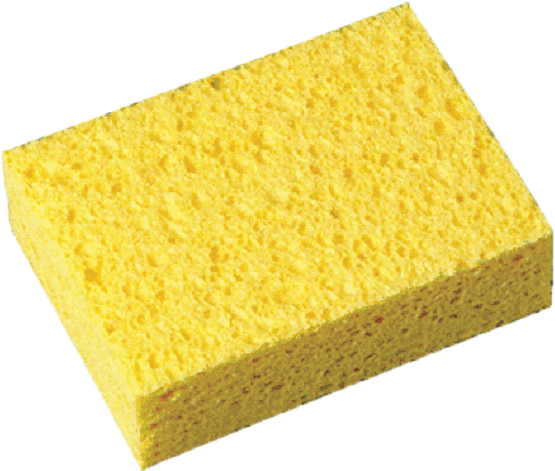
\includegraphics[height=1in]{../images/sponge}
		\end{center}
	\end{block}
\end{frame}
\begin{frame}{\fn}
	\begin{defn}
		If a basis for a vector space $V$ of dimension $n$ is an orthonormal set, then we call it an \emph{orthonormal basis}.
	\end{defn}
	\begin{statementblock}{Theorem 5.11}
		If $B=\{\vec v_1,\vec v_2,\dots,\vec v_n\}$ is an orthonormal basis for an inner product space $V$, then the representation of $\vec w\in V$ in terms of $B$ is given by
			\[\vec w=\ip{\vec w}{\vec v_1}\vec v_1+\ip{\vec w}{\vec v_2}\vec v_2+\cdots+\ip{\vec w}{\vec v_n}\vec v_n.\]
	\end{statementblock}
	\begin{exercise}
		Write $\vec w=(3,-2)$ in terms of $S=\{(\frac{3}{5},\frac{4}{5}),(-\frac{4}{5},\frac{3}{5})\}$, which you proved to be an orthonormal basis for $\R^2$.
	\end{exercise}
\end{frame}
\begin{frame}{\fn}
	\begin{statementblock}{Theorem 5.10}
		If $S=\{\vec v_1,\vec v_2,\dots,\vec v_n\}$ is an orthogonal set of nonzero vectors in an inner product space $V$, then $S$ is linearly independent.
	\end{statementblock}
	\begin{nb}
		In the beginning of the proof of this, we let $c_1,c_2,\dots,c_n$ be scalars such that
			\[c_1\vec v_1+c_2\vec v_2+\cdots+c_n\vec v_n=\vec 0.\]
		You then should use the orthogonality by taking the inner product of $\vec v_i$ with \[c_1\vec v_1+c_2\vec v_2+\cdots+c_n\vec v_n.\]
		for each $i$.
		
		You also make use of the fact that $\langle \vec 0,\vec v\rangle=0$ for all $\vec v$, no matter the inner product space $V$.
	\end{nb}
\end{frame}
\begin{frame}[fragile]
	\frametitle{\fn}
	\begin{exercise}
		Let $S=\{(\frac{3}{5},\frac{4}{5}),(-\frac{4}{5},\frac{3}{5})\}$. Use $\vec v_1=(\frac{3}{5},\frac{4}{5})$ and $\vec v_2(-\frac{4}{5},\frac{3}{5})$. What is
		\begin{enumerate}[label=(\alph*)]
			\item $(3\vec v_1-2\vec v_2)\cdot\vec v_1?$
			\item $(3\vec v_1-2\vec v_2)\cdot \vec v_2?$
			\item $(3\vec v_1-2\vec v_2)\cdot(-\vec v_1+5\vec v_2)?$
		\end{enumerate}
	\end{exercise}
	\begin{nb}
		You can create a vector in Sage \url{http://sagecell.sagemath.org} using
		\begin{verbatim}
		v1 = vector((3/5,4/5))
		v2 = vector((-4/5,3/5))
		v3 = 3*v1-2*v2
		print(f"v3 = {v3}")
		ansa = v3.dot_product(v1)
		print(f"answer to (a) = {ansa}")
		\end{verbatim}
	\end{nb}
\end{frame}
%\begin{frame}{\fn}
%	\begin{statementblock}{Theorem 5.12 (Gram--Schmidt Process)}
%		Let $B=\{\vec v_1,\vec v_2,\dots,\vec v_n\}$ be a basis for an inner product space $V$.
%		
%		Consider $B'=\{\vec w_1,\vec w_2,\dots,\vec w_n\}$ consist of the vectors $\vec w_i$ in $V$ defined by
%			\begin{eqnarray*}
%				\vec w_1 &=&\vec v_1\\
%				\vec w_2 &=& \vec v_2-\proj_{\vec w_1} \vec v_2\\
%				\vec w_2 &=& \vec v_3-\proj_{\vec w_1}\vec v_3-\proj_{\vec w_2} \vec v_3\\
%				&\vdots\\
%				\vec w_n &=& \vec v_n-\proj_{\vec w_1}\vec v_n-\proj_{\vec w_2}\vec v_n- \cdots -\proj_{\vec w_{n-1}}\vec v_n.
%			\end{eqnarray*}
%		Then $B'$ is an orthogonal basis for $V$.
%		
%		Moreover if $\vec u_i=\frac{\vec w_i}{\|\vec w_i\|}$, the unit vector in the direction of $\vec w_i$, then $B''=\{\vec u_1,\vec u_2,\dots,\vec u_n\}$ is a basis for $V$.
%	\end{statementblock}
%\end{frame}
%\begin{frame}{\fn}
%	\begin{exercise}
%		Use the Gram--Schmidt process to find an orthonormal basis for $V=\{(2t+s,3t+s,s,t):s,t\in\R\}$ with respect to the dot product in $\R^4$.
%		\begin{enumerate}[label=(\alph*)]
%			\item Find a basis for $V$, $B=\{\vec v_1,\vec v_2\}$.
%			\item Set $\vec w_1=\vec v_1$.
%			\item Compute $\proj_{\vec w_1} \vec v_2$.
%			\item Set $\vec w_2=\vec v_2-\proj_{\vec w_1} \vec v_2$.
%			\item Find $\vec u_1=\frac{\vec w_1}{\|\vec w_1\|}$ and $\vec u_2=\frac{\vec w_2}{\|\vec w_2\|}$.
%			\item Then $B''=\{\vec u_1,\vec u_2\}$ is an orthogonal basis for $V$.
%		\end{enumerate}
%	\end{exercise}
%\end{frame}
%\begin{frame}{\fn}
%	\begin{exercise}
%		Use the inner product $\ip{\vec u}{\vec v}=2u_1v_1+u_2v_2$ in $\R^2$ and the Gram--Schmidt process to transform $B=\{(2,-1),(-2,10)\}$ into an orthonormal basis for $\R^2$ with respect to this inner product.
%	\end{exercise}
%\end{frame}
\end{document}

